\documentclass[12pt,letterpaper]{article}
\usepackage[utf8]{inputenc}
\usepackage{amsmath, esint}
\usepackage{amsfonts}
\usepackage{amssymb}
\usepackage{listings}
\usepackage{hyperref}
\usepackage[usenames,dvipsnames]{color}
%\definecolor{darkgray}{rgb}{0.3,0.3,0.3}
\usepackage{graphicx} %for pngs
\usepackage[left=1in,right=1in,top=1in,bottom=1in]{geometry}
\author{Nathaniel Beaver}
\title{Goals and use cases for a system that stores, queries, and manipulates equations.}
\begin{document}

\maketitle

\tableofcontents

\section{License}

This work is licensed under the Creative Commons Attribution 3.0 Unported License.
To view a copy of this license, visit \url{http://creativecommons.org/licenses/by/3.0/}.

\section{Motivation}

\begin{quote}
My memory for even the commonest
formulae is poor, and I rely on either reconstructing them or referring to an accepted text.

--- D. J. Finney, "Dimensions of Statistics"
\end{quote}

Equations are ubiquitous in mathematics and science.
However, the way in which we store and reference equations suffers from severe flaws,
such as the inability to transparently manipulate equations,
the difficulty of connecting disparate systems by shared mathematical structure,
and lack of insight into invariance.
This hinders scientific inquiry in a variety of ways.

\section{Use case}

Suppose I want to look up boundary conditions for an electric field to include in a paper I am writing.

\subsection{Print resources.}

Most physicists will reach for their trusty E\&M books in this case.

In the 2nd edition of David J. Griffiths' ``Introduction to Electrodynamics'', for example,
a search of the index for ``Boundary conditions'' gives these equations (in SI units) on page 313:
\begin{align*}
D_{1_\bot} - D_{2_\bot} &= \sigma_f \\
E_{1_\parallel} - E_{1_\parallel} &= 0
\end{align*}

The 3rd edition of John David Jackson's ``Classical Electrodynamics'' also uses SI units,
and a quick check of the index gives:
\begin{align*}
(\mathbf{D}_1 - \mathbf{D}_2)\cdot \mathbf{n} &= \sigma \\
n \times (\mathbf{E}_2 - \mathbf{E}_1) &= 0
\end{align*}

The drawback is that these equations is that they are ``read-only.''
They must be manually typed up for use in a \LaTeX\ document or word processing software,
a laborious process even for relatively short equations.
They are even less suited for use in computational software.

% When you ask a mathematician to come up with a formula to solve a problem,
% you will get something that looks pretty, but that doesn’t mean that it lends
% itself well to computation.
% https://blogs.msdn.microsoft.com/oldnewthing/20130508-00/?p=4423/

Ebooks and PDF files do not solve this problem,
as they do not use \LaTeX\ or computable formats internally.

If the original document is written in \LaTeX\, however,
it is possible to
\href{http://www.ctan.org/pkg/embedfile}
{attach the entire \LaTeX\ source code to a PDF},
although this is somewhat less than convenient for reusing the equation markup,
since it does not automatically unwrap macros into standard \LaTeX\ commands.
This means that the authors must either avoid the use of macros,
or the user must include all necessary packags and copy all the necessary macros to use the equations.

\subsection{Electronic resources.}

Let's see if Wolfram Alpha's database has the boundary conditions.
After all,
it does a good job with
\href{https://www.wolframalpha.com/input/?i=particle+in+a+magnetic+field}
{other equations}.

\url{https://www.wolframalpha.com/input/?i=electric+field+boundary+conditions}

\begin{center}
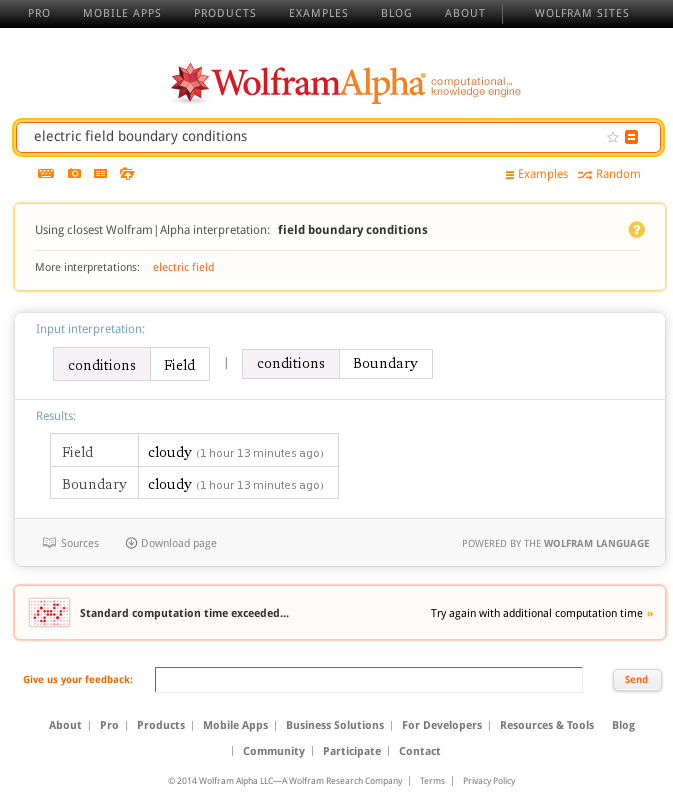
\includegraphics[scale=0.7]{wolfram-alpha-electric-field-boundary-conditions.png}
\end{center}

Hm, that was a little disappointing.

For quick and dirty information finding,
Google works well.
Let's see what the top results are.

\url{https://www.google.com/search?q=electric+field+boundary+conditions}

The
\href{http://farside.ph.utexas.edu/teaching/em/lectures/node59.html}
{first result}, as of \today,
explains their origin from Gauss's Law
and gives the equations as embedded png images:

\begin{center}
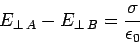
\includegraphics[scale=0.5]{img1337.png}

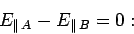
\includegraphics[scale=0.5]{img1344.png}
\end{center}

The
\href{http://www.antenna-theory.com/tutorial/electromagnetics/electric-field-boundary-conditions.php}
{second result} distinguishes between a charged/uncharged surface and uses different notation.
They also use images,
gif in this case
(although I converted them to png for inclusion in this document):
\begin{center}
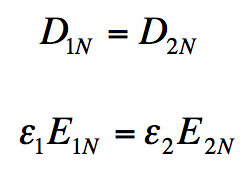
\includegraphics[scale=0.3]{normalDequal.png}
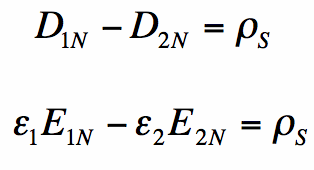
\includegraphics[scale=0.3]{normalEfieldWithCharge.png}
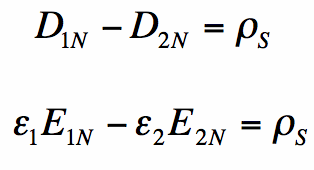
\includegraphics[scale=0.3]{normalEfieldWithCharge.png}
\end{center}

Note that already there is considerable variation in notation.
Furthermore, neither site includes any equations which can be parsed or modified
without first performing optical character recognition on the images;
they are profoundly read-only.

What about
\href{https://en.wikipedia.org/wiki/Interface_conditions_for_electromagnetic_fields}
{Wikipedia}?

This is the relevant equation.

\begin{center}
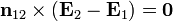
\includegraphics[scale=0.5]{wikipedia1.png}

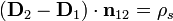
\includegraphics[scale=0.5]{wikipedia2.png}
\end{center}

Fortunately,
there is embedded \LaTeX\ markup available under ``Edit Source''.

\begin{verbatim}
:<math>\mathbf{n}_{12} \times (\mathbf{E}_2 - \mathbf{E}_1)  = \mathbf{0} </math>

:<math>(\mathbf{D}_2 - \mathbf{D}_1) \cdot \mathbf{n}_{12} = \rho_{s} </math>
\end{verbatim}

This will be sufficient for entering into a paper if:
\begin{enumerate}
\item We want \LaTeX\ markup.
\item The Wikipedia editor uses the \LaTeX\ markup correctly.
\item The Wikipedia markup uses the same symbols and units system that we want to use.
\item We only want to typeset the equation, not use it for actual computation.
\end{enumerate}

\section{The problem.}

Both the print and electronic resources have a number of deficiencies.
In particular,
\begin{itemize}
\item Even electronic versions of equations are not generally suitable for using with computational tools.
\item There is no reliable standard for representation of variables,
      even for the simplest and most common equations.
      Sometimes a surface charge is $\sigma$,
      sometimes it is $\sigma_f$,
      and sometimes it is $\rho_s$.
\item There are a variety of different conventions in use that differ between physics and mathematics.
      For example,
      while the right-hand rule is fairly universal,
      the quantities $\phi$ and $\theta$ are
      \href{http://mathworld.wolfram.com/SphericalCoordinates.html}
      {swapped in spherical coordinates}.
      Similar problems exist for
      \href{http://mathworld.wolfram.com/EulerAngles.html}
      {Euler angles}.
\item There are
      \href{https://en.wikipedia.org/wiki/Systems_of_units}
      {many units systems in use in the sciences},
      several of which are popular enough to include in, say, the
      \href{http://lammps.sandia.gov/doc/units.html}
      {software of a given subfield},
      and even if everyone were to standardize tomorrow,
      there are centuries of scholarly literature that is expressed in different units.
      One of the most common examples is the differing forms of equations for SI (MKSA) and Gaussian (cgs) systems.
      There are valid arguments for using either system,
      or using the so-called ``natural units''.
      Converting between these systems, however, is tedious,
      and people should not have to spend much time on it.
\item In much the same way as there are many unit systems,
      there are many equally valid
      \href{https://en.wikipedia.org/wiki/Gauge_fixing}
      {choices of gauge}
      in electrodynamics and a
      \href{https://en.wikipedia.org/wiki/Tensor_notation}
      {proliferation of tensor notations}.
      Dirac notation is another example of an elegant notation
      that is occasionally translated into more familiar notation for some manipulations.
\item Most equations are embedded in a particular coordinate space and vector basis,
      such as the old standbys of Cartesian, cylindrical, or spherical coordinates.
      Often, a problem is much easier to attack in a favorable coordinate system.
      If transformation of coordinate systems was effortless,
      exploring alternatives solutions would become far less time-consuming and laborious.
      (Wouldn't it be fun to try solving something in a non-holonomic basis?)
\item Many derivations in physics rely on substitutions that make the equations unitless,
      yet another related form of the equation that is difficult to find without looking up the original derivation.
      These kinds of change of variables are very common,
      but seldom tabulated systematically.
\item Curves like conic sections have representations in Cartesian coordinates,
      polar coordinates, parametric coordinates, and a variety of other exotic options.
      These can be invaluable for simplifying analysis,
      but looking them up is time-consuming
      and re-deriving them is time-consuming and error-prone.
\item No print or electronic resource is free from errors,
      and not everyone checks the errata page.
      Nor is the errata page always free from errors.
\end{itemize}

Together, these problems can make what should be simple tasks into a chore.
There is frequently unnecessary friction,
for example,
in using results from two different papers,
or collaborating with a colleague who uses a different unit system.
And how many scholars have lost hours of work
by writing a paper with one choice of symbols and units
and then having to change them all for a journal submission?

\section{What the solution should look like.}

Instead of trying to convince everyone to use the same units, gauges, and symbols,
it is saner to leverage the ability of machines to do busywork.

An electronic database of equations with the relevant information could easily translate between any system of units,
and could produce output suitable for any software,
regardless of whether it is intended for use in a Fortran program,
a \LaTeX\ document,
or a web browser.

If a transformation between these forms is non-trivial,
the best thing is simply to have a human provide the input and store them both,
and make them easy to find later.
Rather than attempting to find the ``one true form'' of the equation,
it should simply associate various useful formats.

Furthermore,
it should take free-form input queries that would outpace any or paper index.
It could also outpace a web search by taking advantage of limited input domain.

Queries could include items like common names (``Maxwell equations''),
units of variables
(e.g. ``all equations with the left side in units of force''),
and even algebraic forms (all equations of the form \verb|a x^2 + b x + c|).

Given sufficient heuristics and metadata
(much of which will, admittedly, have to be entered manually),
this is a solvable problem.

Finally, it should be personal and collaborative.
It should be easy to import the standard equations,
but most people have specific, personalized needs,
and collaborate with a relatively small group of people,
so the software should reflect that.

\section{Features}\label{sec:features}

\subsection{Semantic features.}

These are broad requirements that do not specify implementation.

\begin{itemize}
\item Provide a means to write explanatory text for symbols or sub-expressions in the relevant equations,
      which most texts do anyway as a matter of course.
      For example, $\vec{L} = I \vec{\omega}$, where
      $\vec{L}$ is angular momentum,
      $I$ is the moment of inertia, and
      $\vec{\omega}$ is the angular velocity.
\item Search for equations by popular name and subfield.
\item Search for equations by regular expression.
\item Search for equations by the symmetries they obey and mathematical groups they belong to.
\item Enter an equation and get back structurally similar and related equations.
\item Enter some symbols and get equations back that use those symbols.
\item Provide the option to perform simple substitutions
      (so a query for $a+b^2$ could return an equation stored as $x+y^2$,
      and one could specify substitution rules so that it outputs $m + n^2$)
\item Provide the option to search for algebraically equivalent forms
      (e.g. $a(b+c)$ could return $a b + a c$).
      Note that this would only work for equations that had unambiguous computable forms provided,
      so that the software could call,
      e.g. Sage, Maxima, or Mathematica to determine whether or not the forms are algebraically equivalent.
      (MathML renderers and \LaTeX\ compilers will happily typeset algebraically ambiguous or uncomputable gibberish.)
\item Provide the option to search for algebraically equivalent forms with simple substitutions
      (e.g.  $a(b+c)$ could return $ x y + x z$)
\item Provide the ability to search based on units,
      such as all equations with an exponent that has units of radians or degrees, for example.
\item Provide the option to choose units system,
      so that a single equation would have both cgs and SI forms available, for example.
\item Allow extensions to specify new unit systems or gauges.
\end{itemize}

\subsection{Technical design features.}

These are some specific requirements of the implementation.

\begin{itemize}
\item Store equation database locally. Network connectivity must not be required for typical use.
\item Provide the capability to update from network sources and merge in other people's changes,
      as existing distributed version control systems do.
\item Store representations in at least one format of a variety of options
      (Unicode UTF-8 plaintext, \LaTeX, MathML, OpenMath, etc.)
      as well as a way to add more specific forms.
      For example, one might be a \LaTeX\ expression with the vector quantities having arrows like this:
      $\vec{r}$;
      and another with vector quantities bolded like this:
      $\mathbf{r}$.
\item Provide the ability to optionally store and access other formats
      (e.g. Mathematica, MS Word, Matlab code, Fortran code, C code etc.)
\item Call existing software to convert between representations,
      so that not everything has to be converted manually.
      This falls into two categories:
      \begin{enumerate}
      \item Conversions that are essentially just formatting conversions.
            For example, while \LaTeX\ and MathML have some very apparent differences,
            they both require only enough information to typeset an equation,
            not actually evaluate it.
            The automatically generated markup could subsequently be tweaked by hand.
      \item Conversions from a typesetting or markup language like \LaTeX\ or MathML to an expression that can actually be evaluated;
            one that you can plug in numbers and get a numeric result.
            Some equations are simple enough that a conversion to, say, C code is trivial
            -- something just using trig, exponents, and arithmetic functions, for example.
            Others will be sufficiently abstract as to require manual conversion or avoiding a computable format at all.
            (Alternately, a link to some remotely hosted code may be in order;
            \hyperref[itm:linking]{see below}.)
            Incidentally, Stephen Wolfram (of Mathematica fame) had this
            \href{http://www.stephenwolfram.com/publications/recent/mathml/mathml1.html}{to say}
            about this kind of conversion.
                \begin{quote}
                Unlike with ordinary human natural language,
                it is actually possible to take a very close approximation to familiar mathematical notation,
                and have a computer systematically understand it.
                That's one of the big things that we did about five years ago in the third version of Mathematica.
                And at least a little of what we learned from doing that actually made its way into the specification of MathML.
                \end{quote}
      \end{enumerate}
\item Link to internal and external references
      (refer to another equation in the same database,
      jump to a specified page of a local or remote PDF or ebook,
      standard html-style links to  urls of relevant websites or source code implementations,
      digital object identifiers (DOIs),
      bibtex references, etc.) \label{itm:linking}
\end{itemize}

\section{Some objections.}

\subsection{There's more to physics and math than equations, you know.}

Yes, and people did complex math for centuries without nice modern algebraic notation,
but equations do provide a very lovely and compact way to represent relationships between variables.

Once we've got an easy and reliable way to find the equations we want,
we can spend more time reasoning about whether the equation is applicable,
what approximations to make,
what the physical interpretation is,
and how that interpretation squares with experiment and physical intuition.

\subsection{Equations without context are dangerous,
            and people will use them when they are not applicable or assume what they are trying to prove,
            i.e.\ use circular reasoning.}

A valid concern,
which is why it's important to write explanatory text about each symbol
and link to more complete discussions.

In any case, people already misuse equations,
and this is generally because they don't want to put in the effort to look up the context of the equation.
Properly used, this software could help mitigate this problem.

\subsection{Why ``equations'' and not ``expressions'' or ``formulas''?}

This is just nomenclature.

I assume that this software could work for mathematical expressions in general,
identities, approximations, chemical formulas, etc.
Most of the time, though,
we need to know about relationships between variables,
so ``equations'' are what most people think of and use regularly.

\subsection{Making it easier to change conventions will encourage fragmentation.}

Possibly, but it's pretty badly fragmented already.
If there is a reliable system to automatically convert systems of units and other conventions,
fragmentation will not matter as much.

Some fragmentation is due to the difficulty of updating existing bodies of work to match modern improvements,
so a system to make this easier could actually reduce fragmentation.

Furthermore,
such a system would make it possible to use a standard form when writing papers and textbooks,
since everyone could convert to their favorite set of conventions without difficulty.

\subsection{Is it really so much work to use a web search or a book index?}

Yes.

Try doing a
\href{https://www.google.com/search?q=%22L+%3D+r+%C3%97+P%22&oq=%22L+%3D+r+%C3%97+P%22}
{Google search for $L = r \times p$}.
\href{http://symbolab.com/search?origin=suggestion&query=L%3Dr%5Ctimes%20p}
{Symbolab works somewhat better} for this, as does
\href{https://www.google.com/search?&q=%22L+%3D+r+%5Ctimes+P%22&oq=%22L+%3D+r+%5Ctimes+P%22}
{searching for likely \LaTeX\ markup}.

% TODO: add this http://searchonmath.com/result?equation=L+%3D+r+\times+p&page=1
% TODO: http://searchonmath.com/result?equation=r+%3D+2+G+m+%2F+c^2&page=1

This is just a simple example of hard it is to find even a basic equation with relatively few ways to express it.

%TODO add more examples explaining how badly things are broken and why this needs to change

As for books, if you can get everything you need from one book, great.
The ones I need are generally scattered across several books and journal articles,
none of which use the same notation.
Note all books have a good glossary or index.

\subsection{Surely there are people already working on this, or something similar?}

There are some
\href{http://symbolab.com}
{interesting}
\href{http://latexsearch.com/}
{websites}
\href{http://www.dessci.com/en/reference/searching/math-searching.htm}
{out}
\href{http://www.equationsheet.com/}
{there},
but they're more about searching existing websites and scholarly literature
and don't accomplish more than a few of the \hyperref[sec:features]{features mentioned above}.

 %TODO: talk about them in more depth, and include this website:
% http://searchonmath.com/
% https://www.quora.com/Is-there-a-way-to-search-Google-for-a-math-equation?share=1
% http://meta.math.stackexchange.com/questions/12993/what-is-the-best-way-to-search-for-a-math-equation-on-the-internet
% http://meta.math.stackexchange.com/questions/10169/how-to-search-for-a-formula-expression
% http://meta.math.stackexchange.com/questions/5048/how-do-you-search-for-specific-questions


Wolfram Alpha is probably the closest right now,
but its goals are broader than storing equations.
The lack of a local, user-controlled database is probably the biggest problem.
One result of this is a tendency towards only storing the ``one true form'' of an equation.

\href{http://www.w3.org/Math/}
{MathML}
and
\href{http://www.openmath.org/}
{OpenMath} are projects that employ similar ideas,
although MathML is focused mainly on web browsers and OpenMath is still unfinished.
(The OpenMath website lists only 58 members,
many of whom are professors that work on it in their spare time.)

More importantly,
OpenMath is working towards a standard for representing the mathematical objects for computer algebra systems,
not a working piece of software performing the functions mentioned above.

The database of equations could certainly use the OpenMath standard as another representation
--- a reliable, standardized representation ---
but it would not require it to work.

\href{http://www.mathjax.org/}
{MathJax} is doing great things for putting math on the web,
but not so much for storage and retrieval.

There are also efforts to make derivations automatic,
i.e. proof assistants and automated theorem proving.
These efforts are intriguing,
but physicists at any rate are more interested in the equations themselves and where they are applicable
than rigorously defining the mechanism to derive the results.

\subsection{Would people actually use this?}

I would, and I have
\href{http://www.researchgate.net/post/I_am_looking_for_an_equation_database_or_digital_list_of_equations}
{reason to believe}
\href{http://productforums.google.com/forum/#!topic/websearch/lVJiyCSl-xk}
{other people would, too}.

\subsection{This is way too hard.}

It's really not;
\hyperref[sec:ambitious]
{see below} for the actually hard/interesting problems.
The individual components have existed for decades,
they just haven't been tied together yet.
I regularly use a
\href{https://en.wikipedia.org/wiki/Recoll}
{desktop search tool} to index and query my local documents,
but it isn't geared to equations and hence doesn't have the specific features I would like.

\subsection{Talk is cheap. Show me the code/data.}

There is an example of a minimal prototype/proof of concept on GitHub here:

\url{https://github.com/nbeaver/equation-manager-prototype}

\subsection{There are too many equations. Searching them all would be hopeless.}

There number of well-formed formulas is indeed infinite,
(though countably so by Gödel numbering)
but only a finite and relatively tiny subset of them are useful or interesting.

For comparison,
there are a lot of Unicode characters,
and more on the way,
but writing a
\href{https://mail.python.org/pipermail/python-announce-list/2003-April/002183.html}
{program to search for the one you want} is not unusual.
The
\href{http://sources.debian.net/src/unicode/0.9.7/unicode}
{code for querying the database} is pretty simple, too.

\section{More ambitious possibilities.}\label{sec:ambitious}

\subsection{Semantics of representation and elimination of ambiguity.}

Mathematical software is traditionally poor at retaining semantics.
This is sometimes beneficial;
it's easy, for example,
to simulate a universe with physical laws that do not match this universe.
However, some level of semantic information can be retained by,
for example, respecting consistent dimensionality and distinguishing indices from regular variables.

This could alleviate the namespace problem which is rampant in physics.
For example,
introductory kinematics generally uses $m$ for mass and $\mu$ for coefficients of friction.
However, many upper-level mechanics books use $\mu$ for reduced mass.
This can get awkward if you want to use reduced mass in a problem with coefficients of friction.

The problem gets much worse when different subfields of a discipline try to use each other's equations.
(There's only so much subscripts can do to increase the number of unique symbols,
especially if subscripts and superscripts are already used for tensor notation.
There are \hyperref[color-coding]{other ways} to distinguish quantities, however.)

If the dimensions of each quantity were unambiguously specified,
the symbols peculiar to the problem wouldn't matter as much,
and symbol collisions could be detected and averted automatically
if the software had a suitable list of candidates for representing each quantity.

\subsection{Automatically converting existing documents.}

By taking advantage of certain reasonable assumptions,
making simple substitution transformations on, say,
a \LaTeX\ document could be straightforward.
Of more interest to physicists, however,
are more difficult transformations,
such as automatically convert the units from,
say, cgs to SI,
as John David Jackson did for the first 10 chapters of 3rd edition of ``Classical Electrodynamics''.

This is possible to do,
and an equation with sufficient metadata to declare whether it was in Gaussian or MKSA units
could theoretically be translated to the other using a lookup table for each quantity.
In practice,
because of things like \LaTeX\ macros and multiple conventions for cgs units
--- does that equation need a factor of $c$ or $c^2$? ---
automatic conversion tends to be fragile.
Some transformations are best done manually,
or at least semi-manually.

%TODO talk about LateX's strength as an input format,
% not in retaining semantics.
% Even though it would be "better" to use \EulerConstant than just e,
% it defeats the purpose of quick entry for LaTeX.
% http://tex.stackexchange.com/questions/14821/whats-the-proper-way-to-typeset-a-differential-operator

A more promising possibility is to develop and use standards like OpenMath
with the goal of making it trivial to shift between notations and conventions.
This will be largely invisible in terms of form,
but such functionality will make collaboration and reuse easier and more robust.

For example,
a textbook with self-describing unit systems built-in could be used by
an engineering class with customary units,
an introductory physics class with SI units,
or as a supplement to an existing work in cgs units,
all without confusion or tedious manual conversion.

\subsection{Insight into dependency structure.}

Hiding behind every derived equation is a dependency graph leading all the way back to first principles.

Equations that ``know'' how they are derived can be more easily altered to understand which assumptions they require.

Once an equations' ancestry is unambiguously specified,
it becomes trivial to answer questions like,
``Is this equation linear in $\theta$?''
or
``Does this equation require isotropic permittivity?''
or
``Does this equation hold for non-Euclidean geometries?''
or
``How would this equation be different if the sign convention for charge were reversed?''

\subsection{``Fingerprints'' for equivalent mathematical expressions.}

Regardless of the notation used in,
for example,
the Pythagorean theorem,
there are always three independent variables.
There is also always two operations (self-multiplication and addition),
or three if we count equality as an operation.
Also, the commutativity properties means that symmetry groups can be used to describe the equation.

These examples of notation-invariant properties could potentially be tabulated and systematized
as a kind of fingerprint for a large number of commonly-used expressions,
which could make recognizing mathematical patterns easier,
since familiarity with the particular notation and choice of symbols would not be necessary to recognize the pattern.

Ideally the fingerprint would be robust enough to help identify the components of a complex equation's sub-expressions with simpler equations.

For example, an expression of the form
\[ a = \frac{b c}{b +c} \]
will get many physicists thinking about electronics,
since the equivalent expression
\[ \frac{1}{a} = \frac{1}{b} + \frac{1}{c} \]
corresponds to adding resistors in parallel or capacitors in series.
However, the symmetry is obscured somewhat in the first form.

A desirable mathematical fingerprint would bring this pattern out into the open,
and would extend to helping identify sums of any number of reciprocals.

Equation metadata provides insight into what is invariant and fundamental in an equation
and what is an artifact of conventions such as positive and negative charge,
origin, gauge, basis, and orientation (left or right handedness) of a vector space.

\subsection{New ways of seeing and reasoning about equations.}

Once an equation can be parsed into a machine-manipulable format,
there are many possibilities,
including color-coding,
dependency graphs to keep track of which parts depend on a given quantity,
and whether it is separable into functions of the variables it depends on.

For example, Richard Feynman had
\href{https://en.wikipedia.org/wiki/Grapheme-color_synesthesia}
{grapheme-color synesthesia}.

\begin{quote}
``When I see equations, I see the letters in colors – I don't know why.
As I'm talking,
I see vague pictures of Bessel functions from Jahnke and Emde's book,
with light-tan j's,
slightly violet-bluish n's,
and dark brown x's flying around.
And I wonder what the hell it must look like to the students."
\end{quote}

Feynman might have seen something like this.

\newcommand{\nF}{\textcolor{DarkOrchid}{n}}
\newcommand{\xF}{\textcolor{Brown}{x}}
\newcommand{\JF}{\textcolor{Tan}{J}}
\boldmath
\[
\JF_{\nF}(i \xF) \JF_{\nF}'(\xF) - i \JF_{\nF}(\xF) \JF_{\nF}' (i \xF) = 0
\]
\unboldmath

% TODO: link to http://blog.revolutionanalytics.com/2015/09/because-its-friday-visualizing-ffts.html#

\label{color-coding}
With sufficient metadata about an equation,
software could automatically color-code the expression by assigning different colors to
functions and operators,
independent free variables,
dependent free variables,
and bound (a.ka. ``dummy'') variables or indices.

This makes it faster and easier to answer questions like,
``How many degrees of freedom does this equation have?''
or
``How much of this equation could be replaced by a numeric constant?''

\subsubsection{An example coloring scheme for simple equations.}

\boldmath

\newcommand{\op}{\textcolor{Plum}} % functions and operators
\newcommand{\fv}{\textcolor{green}} % free variables
\newcommand{\iv}{\textcolor{red}} % independent variable
\newcommand{\fc}{\textcolor{blue}} % named constants
\newcommand{\bv}{\textcolor{Gray}} % indices and other bound variables
\newcommand{\nt}{\textcolor{black}} % normal text
% The normal text command is necessary for certain cases such as \op{\sum_{}^{}} or \op{\frac{}{}} to return to normal text.

%$\op{a} \fv{a} \iv{a} \fc{a} \bv{a}$

%DONE Color-code these equations.
%DONE Make the equations bold to see the color more easily.

\begin{description}
\item[Well-defined functions and operators] are \op{purple}.
      This includes elementary binary arithmetic operations like $\op{+}$, $\op{-}$, $\op{\times}$, and $\op{\div}$;
      abstractions of them like $\op{\sum}$, $\op{\prod}$, and the $\op{\frac{\hspace{1em}}{\hspace{1em}}}$ in $\op{\frac{\fv{a b}}{\fv{c d}}}$;
      integer-only operations like factorial $\op{!}$ and modulo arithmetic $\fc{5} \equiv \fc{17} \op{ \mod{ \fc{12} }}$
      real-valued functions like $\op{\log}$, $\op{\sin}$, absolute value $\op{|}\fv{x}\op{|}$, and the gamma function;
      vector operations like the cross-product, dot-product, and various $\op{\nabla}$ operations;
      set operations like $\op{\cap}$ and $\op{\cup}$,
      the operators of differential and integral calculus like
      $\op{\lim_{\bv{x} \to \fc{\infty}}}\frac{\op{\sin} \bv{x}}{\bv{x}}$,
      $\op{\int \mathrm{d}}\fv{x}$,
      and
      $\op{\frac{d}{d\fv{x}}}$
      and their complex and vector versions;
      generalized binary operators like the Kronecker delta, Poisson brackets, and commutator brackets;
      and also generalized functions like the Dirac delta function.
      If it acts on zero or more inputs and is well-defined,
      it falls into this category.
\item[Free variables or functions] are \fv{green}. This includes quantities such as $\fv{x}$ and $\fv{n}$ in the binomial approximation $(\fc{1}\op{+}\fv{x})^{\fv{n}} \approx \fc{1} \op{+} \fv{n}\fv{x}$
      and the function $\fv{f}$ in the linear approximation $\fv{f}(\iv{x}) \approx \fv{f}(\fv{a}) + \fv{f}\op{'}(\fv{a})(\iv{x}-\fv{a})$.
      It also includes free constants such as constants of integration.
      If it could have a value or definition but has not been assigned one,
      it falls into this category,
      even if it is later assigned a value or definition.
\item[The independent variable] is \iv{red}.
      The choice of independent variable is not intrinsic to the equation,
      but making it a different color gives context to the intended use of the relation.
      It is a semantic annotation,
      not a rigorously defined construct.

\item[Fixed constants] are \fc{blue}.
      These include numeric constants like $\fc{0}$, $\fc{\pi}$ or $\fc{e}$,
      vector constants like unit vectors $\fc{\hat{x}}$,
      physical constants like the speed of light $\fc{c}$ or Avogadro's number $\fc{N_A}$,
      unchanging sets such as the set of real numbers $\fc{\mathbb{R}}$,
      unchanging groups like the symmetry group of a square $\fc{D_4}$,
      and even poorly defined but fixed abstractions such as $\fc{\infty}$ and $\fc{-\infty}$.
      It does not include constants of integration,
      unless the constant's value is fixed by some constraint.
      If it is a fixed quantity with a single,
      widely accepted definition and a few common representations (ideally only one representation),
      it fits into this category.
      (Note that some physical constants may not actually be constant,
      so this is context-dependent and depends on the author's intent.
      Also note that for these purposes,
      ``constant'' does not include quantities that must be kept constant to make equation valid.
      For example, $\fv{n_1}$ is constant over space in a homogeneous material described by Snell's Law
      $\fv{n_1} \op{\sin} \fv{\theta_1} = \fv{n_2} \op{\sin} \fv{\theta_2}$
      Nevertheless,
      although the relation assumes $\fv{n_1}$ is constant over time and space,
      $\fv{n_1}$ of the entire medium is free to vary,
      so $\fv{n_1}$ is still considered a free variable.
      Similarly,
      while drag coefficients are constant for a given object at a given Reynolds number,
      they are freely variable components of the drag equation.)
\item[Indices and other bound variables] are \bv{gray}.
      This includes $\bv{k}$ in
      $\op{\sum_{\bv{k} \nt{=} \fc{0}}^{\fc{100}}}$
      and $\bv{x}$ in
      $\op{\int_{\fc{0}}^{\fc{2}}} \! \bv{x}^{\op{2}} \, \op{\mathrm{d}} \bv{x}$
      as well as tensor indices.
      If its value is assigned and constrained by an operator in a well-defined way,
      but also varies,
      and the choice of symbol is completely arbitrary,
      it falls into this category.
      Note that the constraint must be explicit and local to the expression;
      most free variables have some kind of constraints on them,
      but not enough to evaluate the expression.
\item[Everything else] remains \nt{black}.
      This includes clarifying parenthesis in expressions like
      $(
        \fv{a} \op{/} \fv{b}
       )\op{/}
       \fv{c}$,
      as well as mathematical shorthand like $\forall$, $\in$, $\subset$, $\therefore$, and relations like $>$, $\geq$, $=$, $\neq$, and $\approx$.
\end{description}

This scheme has many limitations.
For example, it
\begin{itemize}
\item is skewed in favor of equations used by physicists,
not equations used by e.g. statisticians or group theorists;
\item does not distinguish between kinds of operators or functions;
\item does not distinguish between integer-value, real, and complex free variables;
\item does not establish whether free variables depend on other free variables or not;
\item does not explicitly show the implicit multiplication operations;
\item does not separate the operation of raising a value to the $\fv{n}$th power (e.g $\fc{2}^{\fv{n}}$) from the free variable $\fv{n}$.
\item Contains some ambiguities.
      For example, squaring a constant is performing an operation on that constant,
      but the result is still a constant,
      so perhaps the entire thing should be colored as a constant?
\end{itemize}

However, it does have some good points as well. For example,

\begin{itemize}
\item Color is unused by existing notation,
      so any equations can be coded without loss of information.
\item Highlighting the independent variable in \iv{red} conveys the author's intent.
\item An extra degree of freedom for disambiguating expressions. A primed variable $\fv{f'}$ is different from the derivative of a function $\fv{f}\op{'}$.
\item Mental variable collisions are less likely.
      It is easy to distinguish a constant of integration $\fv{c}$ from the speed of light $\fc{c}$.
\item The line between functions and variables is generally not clear-cut,
      since most variables depend on other variables.
      This scheme sidesteps the problem by lumping them together.
\item It increases the information density of an equation without adding excess complexity;
      only five easily distinguishable hues are added.
\item It constitutes a rudimentary visual type system for the expressions,
      which helps catch error and inconsistencies.
      Differentiating with respect to a fixed constant is obviously wrong,
      for example.
\end{itemize}

Here is a small selection of equations codes with this scheme,
mainly selected from calculus (i.e. real analysis) and the physical sciences.

Compton scattering

\[
\fv{\lambda'} \op{-} \fv{\lambda}
=
\op{\frac{\fc{h}}{\fc{m_e} \fc{c}}}
\left(
    \fc{1} \op{-} \op{\cos} \, \iv{\theta}
\right)
\]

Fundamental Theorem of Calculus

\[
\op{\int_{\fv{a}}^{\fv{b}}}
\iv{F}\op{'}(\bv{x})
\op{\mathrm{d}} \bv{x}
=
\iv{F}(\fv{b})
\op{-}
\iv{F}(\fv{a})
\]


Binomial coefficients

\[
\op{
  \binom{
    \fv{n}
  }{
    \iv{k}
  }
}
=
\op{
  \frac{
      \fv{n}\op{!}
  }{
      \iv{k} \op{!}
      \,
      (
        \fv{n} \op{-} \iv{k}
      )\op{!}
  }
}
=
\op{
  \prod_{
    \bv{i} \, \nt{=} \, \fc{1}
  }^{
    \iv{k}
  }
}
\op{
  \frac{
      \fv{n}
      \op{-}
      ( % TODO make these parentheses black
        \iv{k} \op{-} \bv{i}
      )
    }{
      \bv{i}
  }
}
\]

Geometric series
\[
\fv{a}
\op{+} \fv{a}\iv{r}
\op{+} \fv{a} \iv{r}^{\op{2}}
\op{+} \fv{a} \iv{r}^{\op{3}}
\op{+}
\cdots
\op{+} \fv{a} \iv{r}^{\op{\fv{n} \op{-} \fc{1}}}
=
\op{
  \sum_{
    \bv{k} \, \textcolor{black}{=} \, \fc{0}
  }^{
    \fv{n} \op{-} \fc{1}
  }
}
\fv{a} \iv{r}^{\bv{k}}
=
\fv{a}
\,
\op{
  \frac{
    \fc{1} \op{-} \iv{r}^{\fv{n}}
  }{
    \fc{1} \op{-} \iv{r}
  }
}
\]

Gauss' Law

\[
\op{\oint_{\fv{A}}}
\iv{\vec{E}}
\op{\cdot}
\op{\mathrm{d}}
\fv{\vec{A}}
=
\frac{
  \fv{Q_{in}}
  }{
  \fc{\varepsilon_0}
  }
\]

Divergence theorem

\[
\op{\iiint_{\fv{V}}}
  \left(
    \op{\nabla \cdot}
    \iv{\vec{F}}
  \right)
  \,
  \op{\mathrm{d}}
  \fv{V}
=
\op{\oiint_{\fv{S}}}
  \iv{\vec{F}}
  \,
  \op{\cdot}
  \,
  \bv{\vec{n}}
  \,
  \op{\mathrm{d}}
  \fv{S}
\]

Stokes' theorem

\[
\op{\iint_{\fv{S}}}
  \op{\nabla \times}
  \iv{\vec{F}}
  \,
  \op{\cdot}
  \,
  \op{\mathrm{d}}
  \fv{\bv{\vec{S}}}
=
\op{\oint_{\partial \fv{S}}}
  \iv{\vec{F}}
  \cdot
  \op{\mathrm{d}}
  \bv{\vec{r}}
\]

Drag force acting on a projectile

\[
\fv{\vec{F_D}}
=
\op{-}
\iv{\hat{v}}
\fc{\frac{1}{2}}
\fv{C_D}(
  \fv{\iv{v}}
)
\fv{\rho}
\fv{A}
\iv{v}^{\op{2}}
\]

Van der Waals gas:
\[
\left(
  \fv{p}
  +
  \frac{
    \fv{n}^{\op{2}}
    \fv{a}
  }{
    \fv{V}^{\op{2}}
  }
\right)
\left(
  \fv{V}
  \op{-}
  \fv{n}
  \fv{b}
\right)
=
\fv{n}
\fc{R}
\iv{T}
\]

Trapezoidal rule

\[
\op{
  \int_{
    \fv{a}
  }^{
    \fv{b}
  }
}
\! % reduce spacing
\iv{f}(\bv{x})
\, % add extra space
\op{\mathrm{d}} \bv{x}
\approx
(
  \fv{b}
  \op{-}
  \fv{a}
)
\left(
  \frac{
    \iv{f}(\fv{a})
    \op{+}
    \iv{f}(\fv{b})
  }{
    \fc{2}
  }
\right)
\]

Bohr model radius of electron orbit

\[
\fv{r}_{\iv{n}}
=
\op{\frac{
  \iv{n}^{\op{2}}
  \fc{\hbar}^{\op{2}}
}{
  \fv{Z}
  \fc{k_\mathrm{e}}
  \fc{e}^{\op{2}}
  \fc{m_\mathrm{e}}
}}
\]

Rydberg formula for hydrogen

\[
\fv{\lambda}^{\op{-1}}
=
\frac{
  \fc{m_e}
  \fc{e}^{\op{4}}
}{
  \fc{8}
  \fc{\varepsilon_0}^{\op{2}}
  \fc{h}^{\op{3}}
  \fc{c}
}
\left(
  \fv{n_1}^{\op{-2}}
  \op{-}
  \fv{n_2}^{\op{-2}}
\right)
\]

Virial theorem

\[
\fc{2}
\op{
  \left\langle
    \fv{T}
  \right\rangle
}
=
\op{-}
\op{
  \sum_{
    \bv{k} \textcolor{black}{= \fc{1}}
  }^{
    \fv{N}
  }
}
\op{
  \left\langle
    \iv{\vec{F}_{\bv{k}}}
    \op{\cdot}
    \fv{\vec{r}_{\bv{k}}}
  \right\rangle
}
\]

Einstein field equations

\[
\fv{R}_{\bv{\mu} \bv{\nu}}
\op{-}
\op{\frac{\fc{1}}{\fc{2}}}
\fv{g}_{\bv{\mu} \bv{\nu}} \, \fv{R}
\op{+}
\fv{g}_{\bv{\mu} \bv{\nu}} \fc{\Lambda}
=
\op{\frac{\fc{8 \pi G}}{\fc{c^4}}}
\fv{T}_{\bv{\mu} \bv{\nu}}
\]

Fourier transform

\[
\fv{\hat{f}}
  (\fv{\xi})
=
\op{\int_{\fc{-\infty}}^{\fc{\infty}}}
  \iv{f}(\bv{x})
  \ \fc{e}^{\op{-} \fc{2\pi i} \bv{x} \fv{\xi}}
  \,
  \op{\mathrm{d}} \bv{x}
\]

%TODO Fourier transforms
%TODO add links for all these equations

\unboldmath

%TODO Cut down on the number of "could"s, "would"s, and "should"s.



\subsection{Reasoning about physical systems and connections between them based on mathematical structure.}

The practical purpose of associating equivalent forms is to save time and effort.
The greater purpose is to make explicit connections between seemingly disparate systems.

There are many famous examples of the same equation describing seemingly unrelated phenomena.
For example,
the scalar wave equation describes vibrations in both solids and fluids,
and similar equations describe electromagnetic waves and quantum mechanical wavefunctions.
The hydraulic analogy provides a useful and intuitive
(though potentially misleading)
way to reason about electronic circuits.

However,
such connections are not isolated to famous results;
such connections are discovered or rediscovered regularly.
Such connections could be made more quickly and rigorously if governing equations,
symmetries, and boundary conditions were explicitly stated in a way that could be compared to other systems to test for equivalence.

Physicists delight in the rich mathematical structure of the systems they study.
Sadly, they are all too often divided from the mathematicians and from each other by mere notation.
By unifying and linking the language of mathematics,
we can avoid reduplication of effort and make explicit connections which were otherwise unknown or neglected.

\end{document}
